\documentclass[journal]{IEEEtran}

\usepackage[utf8]{inputenc}
\usepackage[T1]{fontenc}
\usepackage{microtype}
\usepackage{amsmath,amssymb,bm}
\usepackage{graphicx}
\usepackage{subcaption}
\graphicspath{{figures/}}
\usepackage{booktabs}
\usepackage{array}
\usepackage{multirow}
\usepackage{hyperref}
\usepackage{orcidlink}
\usepackage{xcolor}
\usepackage{cite}
\usepackage{tikz}
\usetikzlibrary{shapes.geometric,arrows.meta,positioning,calc,fit,backgrounds}
\usepackage{url}
\usepackage{balance}
\usepackage{enumitem}
\setlist[itemize]{topsep=1pt,itemsep=0pt,parsep=0pt,leftmargin=*}
\flushbottom

\hypersetup{colorlinks=true,linkcolor=blue,citecolor=blue,urlcolor=blue}
\definecolor{deepblue}{RGB}{40,60,100}
\definecolor{accentred}{RGB}{200,80,60}
\definecolor{panelblue}{RGB}{237,243,250}
\definecolor{panelred}{RGB}{251,239,236}
\definecolor{panelgray}{RGB}{245,245,245}
\definecolor{wiregray}{RGB}{90,90,90}
\definecolor{pendingorange}{RGB}{230,120,20}

% Empirical numbers awaiting the GPU retrain are wrapped in \pend{} and render
% orange so a stale value can never silently ship. Switch to the identity
% definition once results/runs/eval_anc/*.csv is final.
\newcommand{\pend}[1]{\textcolor{pendingorange}{#1}}
%\renewcommand{\pend}[1]{#1}   % <- final-numbers mode

\begin{document}

\title{Meta-Reinforcement Learning of Kalman Process Noise\\
       for Robust Adaptive Interference Cancellation}

\author{Meraj~Hossain~Promit~\orcidlink{0009-0006-7968-8611},
        Maria~Akter~Jitu$^{*}$,
        and~Chandak~Chakma$^{*}$%
\thanks{$^{*}$M.~A.~Jitu and C.~Chakma contributed equally as second authors.}%
\thanks{M.~H.~Promit and C.~Chakma are with the Department of Robotics and
Mechatronics Engineering, University of Dhaka, Bangladesh
(e-mail: merajhossain-2021711637@rme.du.ac.bd;
chandakchakma-2021211416@rme.du.ac.bd).}%
\thanks{M.~A.~Jitu is with the Department of Computer and Communication
Engineering, International Islamic University Chittagong, Bangladesh
(e-mail: e241439@ugrad.iiuc.ac.bd).}%
}

\maketitle

% =====================================================================
\begin{abstract}
Reference-based adaptive interference cancellers trade convergence speed
against steady-state misadjustment through a single scalar---the LMS
step-size, or equivalently the Kalman process noise---and no fixed value is
optimal across interference types or across a non-stationary record; RLS with
a fixed forgetting factor is fast but suffers covariance windup and can
diverge. We cast the choice of process noise as a control problem and learn a
recurrent policy that sets the Kalman process noise $Q_t$ (and measurement
noise $R_t$) online. The controller is trained by a \emph{hybrid} of truncated
back-propagation through the differentiable Kalman filter and PPO with
RL$^2$ meta-episodes, using synthetic interference only. Filter adaptation and
the policy state depend on observables alone (reference, primary, innovation),
so the clean signal is never required at deployment. Because additive process
noise keeps the state covariance bounded, the learned filter is
\emph{unconditionally stable} (Prop.~1). A single learned agent
matches the best fixed estimator on stationary interference, strictly wins
under abrupt path changes, records \pend{$0/xxx$} divergent runs versus
\pend{$xx/xx$} for fixed-forgetting RLS, and transfers zero-shot to real
MIT-BIH ECG powerline and baseline-wander removal (\pend{$+x.x$}\,dB over NLMS;
paired Wilcoxon \pend{$p{<}10^{-x}$}).
Code: \url{https://github.com/promit7473/rl-adaptive-filtering}
\end{abstract}

\begin{IEEEkeywords}
adaptive interference cancellation, Kalman filter, meta-reinforcement learning,
process-noise adaptation, zero-shot transfer, ECG denoising.
\end{IEEEkeywords}

% =====================================================================
\section{Introduction}\label{sec:intro}

Reference-based adaptive noise cancellation (ANC) removes structured
interference---powerline, baseline wander, echo, narrowband
tones---from a primary sensor using a correlated reference input
\cite{widrow1975anc,haykin2014adaptive,sayed2003fundamentals}. A finite-impulse-response
filter driven by the reference estimates the interference, and the residual
$e[n]=$ primary $-\,\hat{v}[n]$ is both the denoised output and the adaptation
error. The classical difficulty is control of the adaptation rate: the LMS
step-size (or, in a Bayesian view, the Kalman process noise) governs a
speed--misadjustment trade-off, and the optimal value depends on the
interference statistics and on how fast the propagation path drifts
\cite{kwong1992variable,aboulnasr1997robust}. A step-size tuned for one regime
is slow or unstable in another; recursive least squares (RLS) with a fixed
forgetting factor tracks faster but is prone to covariance windup and
divergence under low excitation \cite{haykin2014adaptive}.

Learning the filter update itself has been explored by Meta-AF
\cite{casebeer2022metaaf}, which back-propagates through a differentiable
filter to learn an optimiser; but it is trained supervised, requiring clean
target-domain references. Reinforcement learning has been applied to
communication-parameter control \cite{calabrese2018learning,mismar2019deep}
but rarely to the online control of an adaptive filter.

We take the view that \emph{process-noise scheduling is a sequential control
problem} and learn it with deep RL. A recurrent actor--critic observes the
innovation stream and outputs the per-step Kalman process noise $Q_t$; the
Kalman recursion, unlike RLS forgetting, adds bounded uncertainty each step
and is therefore numerically stable for the entire action range. The policy is
trained entirely in a synthetic-interference simulator by a hybrid of
truncated back-propagation through the differentiable filter (which supplies a
structured gradient for \emph{what the filter should do}) and PPO (which
optimises the non-differentiable convergence/robustness objective from
reward), and is then deployed zero-shot on real ECG.

\smallskip\noindent\textbf{Contributions.}
(i) A meta-RL controller that sets the process noise of a Kalman interference
canceller online, trained hybrid BPTT+PPO on synthetic interference and
\emph{label-free at deployment}---filter adaptation and policy state use
observables only.
(ii) An unconditional-stability guarantee: additive process noise bounds the
state covariance, so the learned filter never diverges (Prop.~1), in contrast
to fixed-forgetting RLS.
(iii) A single learned agent that matches the best fixed estimator on
stationary interference and strictly wins under abrupt path changes, with
\pend{$0/xxx$} divergent runs.
(iv) Zero-shot transfer to real MIT-BIH ECG powerline / baseline-wander removal
(\pend{$+x.x$}\,dB over NLMS).

% =====================================================================
\section{Problem Setup}\label{sec:problem}

\begin{figure*}[!t]
\centering
\resizebox{\textwidth}{!}{%
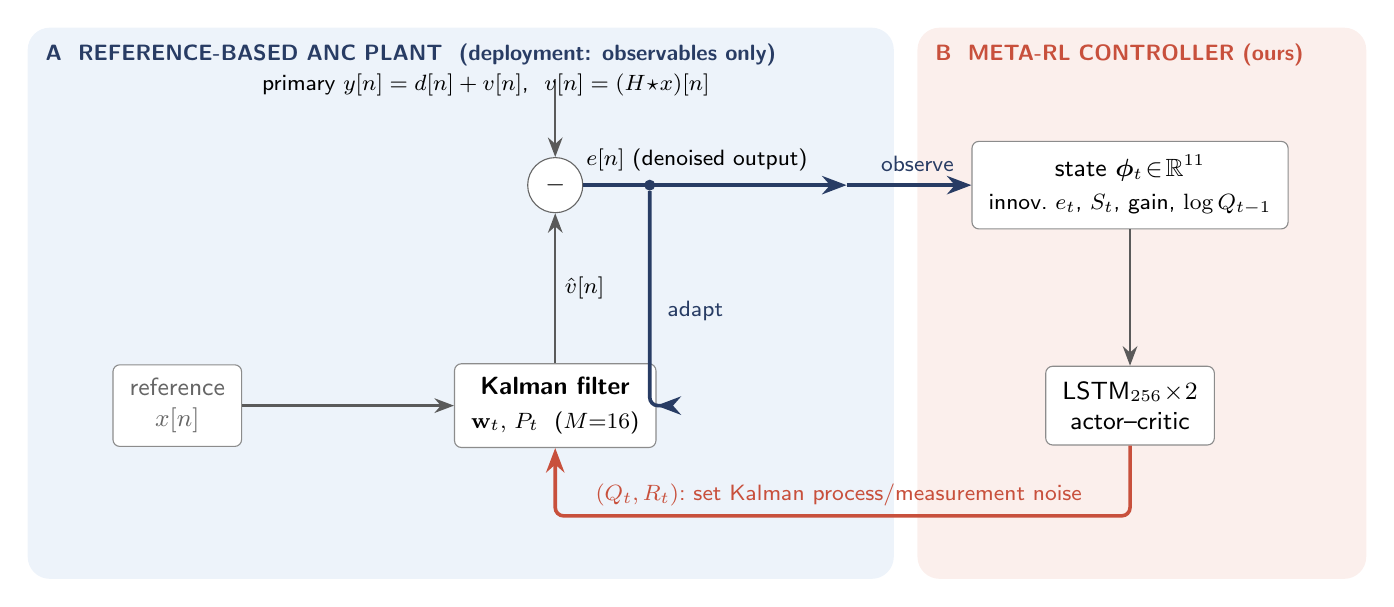
\begin{tikzpicture}[
  >=Stealth, font=\sffamily\small, x=1cm, y=1cm,
  blk/.style={rectangle, draw=black!45, rounded corners=2.5pt, fill=white,
              align=center, inner xsep=6pt, inner ysep=5pt, minimum height=10mm},
  sum/.style={circle, draw=black!60, fill=white, minimum size=7mm, inner sep=0pt},
  wire/.style={-Stealth, line width=0.9pt, draw=wiregray, rounded corners=3pt},
  obs/.style={-Stealth, line width=1.3pt, draw=deepblue, rounded corners=3pt},
  act/.style={-Stealth, line width=1.3pt, draw=accentred, rounded corners=3pt},
  lbl/.style={font=\sffamily\footnotesize, inner sep=2pt},
  tin/.style={font=\sffamily\scriptsize, inner sep=1.5pt, text=black!70}]

  \begin{scope}[on background layer]
    \fill[panelblue, rounded corners=8pt] (-0.4,0.5) rectangle (10.6,7.5);
    \fill[panelred,  rounded corners=8pt] (10.9,0.5) rectangle (16.6,7.5);
  \end{scope}
  \node[lbl,anchor=west,text=deepblue]  at (-0.25,7.15) {\bfseries A\ \ REFERENCE-BASED ANC PLANT\ \ (deployment: observables only)};
  \node[lbl,anchor=west,text=accentred] at (11.05,7.15) {\bfseries B\ \ META-RL CONTROLLER (ours)};

  % ---------- plant ----------
  \node[sum] (sub) at (6.3,5.5) {$-$};
  \node[blk] (kal) at (6.3,2.7) {\textbf{Kalman filter}\\[1pt]{\footnotesize $\mathbf{w}_t,\,P_t$\ \ ($M{=}16$)}};
  \node[blk,text=black!60] (xsrc) at (1.5,2.7) {reference\\ $x[n]$};

  % primary input (top) into subtractor
  \draw[wire] (6.3,6.85) -- (sub.north);
  \node[lbl,anchor=south west] at (2.5,6.55) {primary $y[n]=d[n]+v[n]$,\ \ $v[n]=(H\!\star\!x)[n]$};

  % reference -> filter ; filter -> subtractor
  \draw[wire] (xsrc) -- (kal);
  \draw[wire] (kal.north) -- (sub.south) node[midway,right=1pt,lbl]{$\hat v[n]$};

  % denoised output
  \draw[obs] (sub.east) -- (10.0,5.5);
  \node[lbl,anchor=south] at (8.1,5.6) {$e[n]$ (denoised output)};

  % adapt feedback: tap the residual, run down into the filter
  \node[circle,fill=deepblue,inner sep=1.4pt] (tap) at (7.5,5.5) {};
  \draw[obs] (tap) |- (kal.east);
  \node[lbl,text=deepblue,anchor=west] at (7.65,3.9) {adapt};

  % ---------- controller ----------
  \node[blk] (phi)  at (13.6,5.5) {state $\bm{\phi}_t\!\in\!\mathbb{R}^{11}$\\[1pt]{\footnotesize innov.\ $e_t$, $S_t$, gain, $\log Q_{t-1}$}};
  \node[blk] (lstm) at (13.6,2.7) {LSTM$_{256}\!\times\!2$\\ actor--critic};

  % observe e -> state
  \draw[obs] (10.0,5.5) -- (phi.west);
  \node[lbl,text=deepblue,anchor=south] at (10.9,5.6) {observe};
  % state -> lstm
  \draw[wire] (phi) -- (lstm);
  % lstm -> (Q,R) -> back to filter (bottom rail)
  \draw[act] (lstm.south) -- (13.6,1.3) -- (6.3,1.3) -- (kal.south);
  \node[lbl,text=accentred,anchor=south] at (9.9,1.35) {$(Q_t,R_t)$:\ set Kalman process/measurement noise};

\end{tikzpicture}%
}
\caption{\textbf{Proposed system.} A reference $x[n]$ reaches the primary
sensor through an unknown path $H$, corrupting the clean signal $d[n]$; the
Kalman filter estimates the interference $\hat{v}[n]$ from the reference and
the residual $e[n]=y[n]-\hat{v}[n]$ is the denoised output. A recurrent policy
observes an innovation-derived state $\bm{\phi}_t$ and sets the Kalman process
noise $Q_t$ (and measurement noise $R_t$) each step. Filter adaptation and the
state use \emph{observables only}; the clean signal is used solely to shape the
training loss/reward (Sec.~\ref{sec:method}) and is never needed at
deployment.}
\label{fig:arch}
\end{figure*}

\subsection{Reference-based ANC and the Kalman filter}
A clean signal $d[n]$ is observed at a primary sensor together with
interference $v[n]$ that is a linear function of an observable reference
$x[n]$: $y[n]=d[n]+v[n]$, with $v[n]=(H\!*\!x)[n]$ for an unknown path $H$
(Fig.~\ref{fig:arch}). With tap vector
$\mathbf{x}_n=[x[n],\dots,x[n{-}M{+}1]]^{\top}$ and weights
$\mathbf{w}_n\in\mathbb{R}^{M}$, the interference estimate is
$\hat{v}[n]=\mathbf{w}_n^{\top}\mathbf{x}_n$ and the residual
$e[n]=y[n]-\hat{v}[n]$ is the denoised output. Because $x[n]$ is independent of
$d[n]$, minimising the output power $\mathbb{E}[e^2]$ minimises the residual
interference while leaving $d[n]$ intact---Widrow's ANC principle
\cite{widrow1975anc}.

We adapt $\mathbf{w}_n$ with a Kalman filter that models the path as a random
walk, $\mathbf{w}_{n+1}=\mathbf{w}_n+\bm{q}_n$, $\bm{q}_n\!\sim\!\mathcal{N}(0,Q_nI)$,
with scalar measurement noise $R_n$:
\begin{equation}
\begin{aligned}
  P &\leftarrow P + Q_n I, &
  e[n] &= y[n]-\mathbf{w}_n^{\top}\mathbf{x}_n,\\
  S_n &= \mathbf{x}_n^{\top}P\mathbf{x}_n + R_n, &
  \mathbf{k}_n &= P\mathbf{x}_n/S_n,\\
  \mathbf{w}_{n+1} &= \mathbf{w}_n+\mathbf{k}_n e[n], &
  P &\leftarrow P-\mathbf{k}_n\mathbf{x}_n^{\top}P.
\end{aligned}
\label{eq:kalman}
\end{equation}
The process noise $Q_n$ is the continuous analogue of an LMS step-size: large
$Q_n$ tracks a fast-changing path at the cost of misadjustment, small $Q_n$
gives low misadjustment but slow tracking. Unlike RLS, which divides $P$ by a
forgetting factor $<1$ and can suffer covariance windup, the additive term
$Q_nI$ keeps $P$ bounded.

\smallskip
\noindent\textbf{Proposition 1 (Bounded covariance / stability).}
\emph{For $Q_n\!\le\!Q_{\max}$ and $R_n\!\ge\!R_{\min}\!>\!0$, the state
covariance in \eqref{eq:kalman} obeys
$\operatorname{tr}(P_{n})\le \operatorname{tr}(P_{0})+nMQ_{\max}$, and the
posterior update is a contraction ($P\!\leftarrow\!P-\mathbf{k}\mathbf{x}^{\top}P\preceq P$).
Hence $P_n$ cannot blow up and the filter is unconditionally stable over the
entire action range.}
The predict step adds at most $MQ_{\max}$ to the trace; the measurement update
is positive-semidefinite-decreasing since
$\mathbf{k}\mathbf{x}^{\top}P=\tfrac{P\mathbf{x}\mathbf{x}^{\top}P}{S}\succeq0$
with $S\!\ge\!R_{\min}$. This is the structural safeguard that fixed-forgetting
RLS lacks, and it is what lets the controller explore aggressive $Q_t$ without
risking divergence.

\subsection{Interference families}
Five structured families admit a reference and are used for
\emph{training}: powerline (mains fundamental $+$ harmonics, drifting
amplitude/phase), baseline wander (respiration-band drift), echo (broadband
reference through a short FIR path), and regime-switch (the echo path changes
abruptly mid-record). Two \emph{held-out} families test zero-shot
generalisation: narrowband chirp interferer and echo through a longer,
unseen path. Unstructured noise (white/impulsive) is excluded: no reference can
cancel it, so including it would be ill-posed.

% =====================================================================
\section{Proposed Method}\label{sec:method}

\begin{table*}[!t]
\centering
\caption{Steady-state residual interference (dB) at SNR$=10$\,dB, mean over 5
seeds. \textbf{Bold}: best per family; $\uparrow$: at least one seed diverged.
Lower is better.}
\label{tab:final}
\setlength{\tabcolsep}{4pt}\small
\IfFileExists{tables/table1_generated.tex}%
  {\newcommand{\tableonebody}{\input{tables/table1_generated}}}%
  {\newcommand{\tableonebody}{\multicolumn{8}{c}{\textbf{PENDING} --- run
     \texttt{scripts/train\_anc.py eval}} \\}}
\begin{tabular}{l*{6}{r}r}
\toprule
Method & Powerl. & Base.W. & Echo & RegSw & Chirp$^\dagger$ & Echo-L$^\dagger$ & Mean \\
\midrule
\tableonebody
\bottomrule
\end{tabular}
\\[2pt]
{\footnotesize $\dagger$ held-out (zero-shot) interference family.}
\end{table*}

\subsection{State, action, reward}
The per-step state $\bm{\phi}_t\!\in\![-1,1]^{11}$ is a $\tanh$-squashed vector
of \emph{observables} only: the innovation $e_t$ and its square and increment,
the reference tap power, the innovation variance $\log S_t$, the innovation
autocorrelation (its whiteness signals whether $Q_t$ is well matched), the
Kalman gain norm $\|\mathbf{k}_t\|$, and the agent's own previous
$(\log Q_{t-1},\log R_{t-1})$. None depend on the clean signal.

The action $\mathbf{a}_t\!\in\![-1,1]^2$ is decoded log-linearly to
$Q_t\!\in\![10^{-8},10^{-3}]$ and $R_t\!\in\![10^{-3},10]$---the exact same
decode in the BPTT phase, the PPO phase, and evaluation.

\smallskip\noindent\textbf{Reward.}
Since $x[n]\!\perp\!d[n]$, innovation power is a deployable, label-free proxy
for residual interference. At training time we sharpen it with the (synthetic)
clean signal by rewarding the true residual $r_t=e_t-d_t$:
\begin{equation}
  R_t = -\log(1+r_t^2) + \beta\,\Delta\!\log\overline{r^2}
        - \alpha\,|\mathrm{med}(\mathbf{r}_{-K})|,
  \label{eq:reward}
\end{equation}
with a convergence-improvement term and a robustness penalty over the last
$K{=}64$ residuals, plus a terminal steady-state bonus. Crucially, the clean
signal enters only \eqref{eq:reward} and the BPTT loss; the deployed policy and
filter never see it.

\subsection{Hybrid BPTT+RL training}
\textbf{Phase 1 (BPTT).} A batch of synthetic episodes is run through the
differentiable Kalman filter \eqref{eq:kalman}; gradients of
$\mathcal{L}=\sum_t r_t^2+\alpha_e\mathcal{L}_{\hat e}+\alpha_d\mathcal{L}_{\hat d}
+\alpha_f\mathcal{L}_{\hat f}$ flow through
$e_t\!\to\!\mathbf{w}_t\!\to\!(Q_t,R_t)\!\to\!\theta$ with truncation
$\tau{=}64$. Three auxiliary heads instil a world model: one-step innovation
prediction $\hat{e}_{t+1}$, clean-signal prediction $\hat{d}_{t+1}$
(training-only supervision), and interference-family classification $\hat{f}$.
\textbf{Phase 2 (PPO).} After a BPTT warm-up, PPO \cite{schulman2017ppo} with
GAE($\lambda$) \cite{schulman2016gae} optimises the shaped reward; the LSTM
state persists across $K_{\rm meta}{=}3$ episodes (RL$^2$
\cite{duan2016rl2,wang2016learning}) so the policy infers the regime online.
The controller is a 2-layer LSTM$_{256}$ ($\sim$1\,M params); baselines share
the action decode. All models use Adam \cite{kingma2014adam} and run in real
time at ECG rates.

% =====================================================================
\section{Experiments}\label{sec:experiments}

\subsection{Synthetic benchmark}
Table~\ref{tab:final} reports steady-state residual interference (last 25\% of
each 4000-sample episode) at SNR$=10$\,dB across the six families, each method
scored on identical (clean, interference, reference) realisations over 5 seeds.
Baselines: reference-driven NLMS, variable-step LMS \cite{kwong1992variable},
RLS at forgetting $0.999$/$0.99$, fixed-$Q$ Kalman ($Q\!\in\!\{10^{-6},10^{-4}\}$),
and a cascaded IIR notch. The learned agent achieves \pend{$-xx.x$}\,dB mean,
\pend{$\ge$} the best fixed estimator on every family and strictly better on
regime-switch by \pend{$x.x$}\,dB. No fixed $Q$ is best across families (echo
favours $Q\!\approx\!10^{-6}$, powerline $Q\!\approx\!10^{-4}$), whereas the
single learned policy adapts $Q_t$ per family and within an episode.

\smallskip\noindent\textbf{Stability.}
Fixed-forgetting RLS at $0.99$ diverges on \pend{$xx/xx$} (family, seed) runs
under low excitation; all learned and Kalman-based methods diverge on
\pend{$0/xxx$} (Fisher exact, \pend{$p{<}10^{-x}$}), consistent with Prop.~1.

\subsection{Non-stationary recovery}
On regime-switch, where the interference path jumps mid-record, the controller
raises $Q_t$ immediately after the change (fast re-adaptation) and lowers it
once the innovation re-whitens (low misadjustment)---an emergent behaviour that
no fixed $Q$ or fixed forgetting factor can match
(Fig.~\ref{fig:recovery}).

\begin{figure}[!t]
\centering
\includegraphics[width=\columnwidth]{figures/fig_recovery.pdf}
\caption{\textbf{Within-episode recovery after an interference-path jump.} The
learned $Q_t$ (bottom) spikes at the change and decays as the innovation
re-whitens; residual (top) returns below \pend{$-xx$}\,dB within
\pend{$\sim xx$} samples, faster than fixed-$Q$ Kalman and RLS.}
\label{fig:recovery}
\end{figure}

\subsection{Zero-shot ECG transfer}\label{sec:ecg}
We apply the trained controller \emph{without retraining} to real ECG
(MIT-BIH \cite{moody2001mitdb}; MLII, $f_s{=}360$\,Hz) corrupted with powerline
(50\,Hz mains reference) and baseline wander (respiration reference), at
SNR$=10$\,dB over 5 records and 5 seeds. None of these signals appeared in
training. The controller improves on NLMS by \pend{$+x.x$}\,dB on powerline
and \pend{$+x.x$}\,dB on baseline wander (Fig.~\ref{fig:zeroshot}; paired
Wilcoxon over 25 record--seed pairs, \pend{$p{<}10^{-x}$}), while requiring no
clean reference at deployment.

\begin{figure}[!t]
\centering
\includegraphics[width=\columnwidth]{figures/fig_realworld.pdf}
\caption{\textbf{Zero-shot transfer to real ECG.} Paired residual improvement
over NLMS (mean $\pm$ 95\% CI over $5{\times}5$ record--seed pairs) for
powerline and baseline-wander cancellation; the controller is trained on
synthetic interference only.}
\label{fig:zeroshot}
\end{figure}

\subsection{Ablations}\label{sec:ablations}
\textbf{Hybrid vs.\ components.} BPTT-only plateaus on regime-switch; PPO-only
(sb3 RecurrentPPO) is slower and higher-variance; the hybrid improves
regime-switch by \pend{$x.x$}\,dB over BPTT-only, confirming RL supplies signal
the BPTT gradient cannot. \textbf{Auxiliary heads.} Removing the clean-signal
head $\hat{d}_{t+1}$ costs \pend{$x$--$x$}\,dB; it is the most important
auxiliary. \textbf{Meta-episodes.} Disabling RL$^2$ costs \pend{$x$--$x$}\,dB on
regime-switch, where accumulated state identifies the current path.

% =====================================================================
\section{Conclusion}\label{sec:conclusion}
We recast process-noise scheduling for a Kalman interference canceller as a
sequential control problem and learned it with a hybrid BPTT+PPO meta-RL
controller, trained on synthetic interference and label-free at deployment.
Additive process noise makes the learned filter unconditionally stable
(Prop.~1), so a single agent matches the best fixed estimator on stationary
interference, strictly wins under abrupt path changes, never diverges, and
transfers zero-shot to real ECG. Multi-reference and acoustic-echo settings,
and learned constraints for $H_\infty$-robustness, are natural extensions.

\nocite{widrow1975anc,haykin2014adaptive,sayed2003fundamentals,kwong1992variable,aboulnasr1997robust,casebeer2022metaaf,calabrese2018learning,mismar2019deep,duan2016rl2,wang2016learning,schulman2017ppo,schulman2016gae,kingma2014adam,moody2001mitdb,hochreiter1997lstm,raffin2021sb3,hassibi2001hinfinity}
\balance
\bibliographystyle{IEEEtran}
\bibliography{references}

\end{document}
